% !TeX program = pdflatex
% !TeX root = ../main.tex

%*******************************************************
% Ringraziamenti
%*******************************************************
\cleardoublepage
\phantomsection
\pdfbookmark{Acknowledgments}{acknowledgments}

\chapter*{Ringraziamenti}
\markboth{\spacedlowsmallcaps{Acknowledgments}}%
	{\spacedlowsmallcaps{Acknowledgments}}
\thispagestyle{empty}

%\vspace*{-20pt}

%\begin{flushright}{\slshape    
%	Lorem ipsum dolor sit amet, consectetuer adipiscing elit. \\
%	Ut purus elit, vestibulum ut, placerat ac, adipiscing vitae, felis. \\
%	Curabitur dictum gravida mauris.} \\ \medskip
%    --- Donald Ervin Knuth
%\end{flushright}

%\lipsum[1]

\vspace{5pt}

Voglio ringraziare tutte le persone che mi hanno aiutato direttamente e indirettamente non solo alla realizzazione di questo lavoro, ma anche, e soprattutto, nello svolgimento della mia carriera universitaria.

\begin{itemize}
	\item Prima di tutti Viviana, con cui ho vissuto gomito a gomito questi anni e che mi ha sostenuto nei momenti di sconforto, rari, ma sono stati ugualmente la parte più difficile del percorso;
	\item i miei familiari, che mi hanno supportato, e in cima alla lista i miei genitori, che mi hanno sempre dato la possibilità di scegliere la carriera che preferivo in piena libertà, e comunque mi sono rimasti vicino in ogni situazione, offrendomi il loro completo appoggio;
	\item gli amici con cui ho condiviso questi anni di Fisica, in particolare i compagni con cui ho vissuto assieme in Normale, e con i quali sono sopravvissuto fino in fondo, aiutandoci l'un l'altro dall'inizio alla fine;
	\item non di meno anche gli altri amici con cui sono partito da più lontano, e che, sebbene io non mantenessi così frequentemente i contatti, non mi hanno mai dimenticato di anno in anno;
	\item gli altri compagni in Normale, in particolare quelli che sono stati più avanti nel percorso, che mi hanno sempre aiutato, soprattutto dandomi utili consigli dalla loro esperienza;
	\item i professori che mi hanno guidato, in particolare il mio relatore che ha fatto la parte più grossa, ma anche gli altri che hanno contribuito alla mia crescita e alla mie scelte.
\end{itemize}

Tutte queste persone hanno fatto parte della mia vita in qualche modo nei cinque anni in cui ho studiato Fisica all'Università di Pisa, e, nel bene e nel male, senza di loro la mia carriera e il mio percorso sarebbero stati banalmente diversi.

Non in tutti i momenti avrei desiderato che le cose fossero come di fatti erano, ma complessivamente non avrei voluto niente di diverso da ciò che ho avuto, ed è per questo motivo che sono grato alle persone che ho menzionato.

\bigskip
 
\noindent\textit{\myLocation, \MakeTextLowercase{\myTime}}

\smallskip
\vspace*{-20pt}

\begin{flushright}
	\begin{tabular}{m{5cm}}
		\\ \hline
		\centering\myName \\
	\end{tabular}
\end{flushright}

\pagebreak

\vfill

\begin{figure}
	\centering
	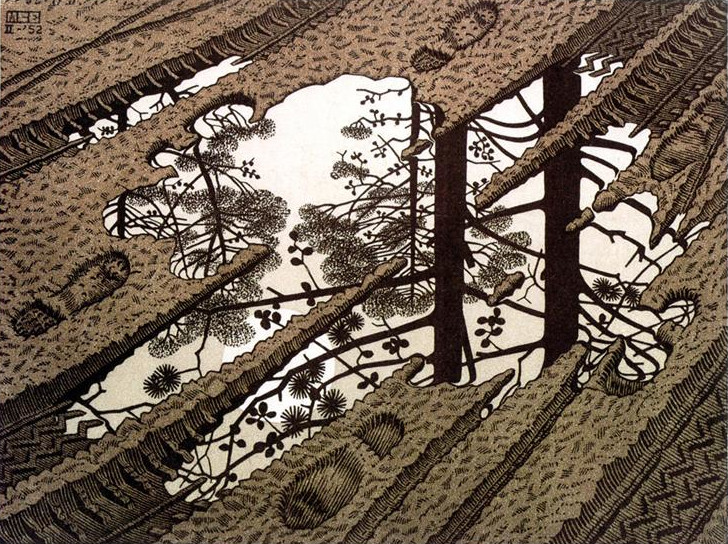
\includegraphics[width=0.9\textwidth]{puddle}
\end{figure}

\vfill
